\documentclass{report}
\usepackage[utf8]{inputenc}
\usepackage{graphicx}
\usepackage{titlesec}
\usepackage{float}

\titleformat{\chapter}[block]
{\normalfont\huge\bfseries}{}{0pt}{\huge}
\titlespacing*{\chapter}{0pt}{-60pt}{20pt}

\title{PRJ3-Article}
\author{J. Brockmöller, J. Gruschka, M. Sajonz, T. Weigand}
\date{January 2021}

\begin{document}
    \maketitle
    \newpage

    \chapter{Overview}


    \section{Introduction}
    The purpose of this article is to describe the functionalities of the Traffic Control System which is implemented in PRJ3 by group 7.
    The article is split into two chapters. At first a general overview of the entire project is given and the architecture and patterns that are used are explained. These patterns can be found illustrated in the last chapter. The second chapter will include a short description of the each member´s work.

    \section{Architecture}
    The project is build with a layered architecture that separates GUI, Business Logic, a main assembler which starts the application and a Persistence Layer which is not required for this project.\\
    To achieve that structure we created different modules for each layer.

    \section{Design Patterns}
    Based on the requirement that a traffic light should be able to switch between different light shapes and colors depending on the country we chose to use the strategy-head-first pattern to encapsulate each behaviour of a traffic light in its own class that implements the interface of the basic light behaviour. The general functions that pedestrian and car lights share are instantiated in the ILight interface which is then extended by a separate interface for each the car light and the pedestrian light behaviour. Country specific behaviours are then implemented in a separate class which implements iLight interface. This pattern is used to switch between different algorithms during run-time. (Fig. \ref{fig:strategyPattern}).\\
    In this particular case these different algorithms are the light behaviours from different countries. A related pattern used in this was the command pattern. This pattern can be used to control the behaviour of others in contrast to the strategy pattern which controls the behaviour of itself. In this project this pattern is used to control the behaviour of the different types of crossings like a simple crossing or a four way crossing (Fig. \ref{fig:commandPattern}).\\
    The third and fourth patterns that are used in this project are the factory pattern and the abstract factory pattern. An abstract light factory which is implemented by an individual factory class for pedestrian lights and car lights which then create country specific traffic lights. In addition the crossing factory is a single factory that creates different kinds of crossings independently(Fig. \ref{fig:factoryPattern}).
    To secure the intended functionality that the traffic lights can be switched dependent on each other we used the observer pattern. For example if the pedestrian traffic light switches on green the car traffic lights switches to red. This pattern is used to notify every observer that is registered as a observer in the regarding subject (Fig. \ref{fig:observerPattern}). This pattern was first only text based implemented and later added to the GUI.

    \chapter{Personal Parts}

    \section{Tim Weigand}

    Due to the fact that we did a lot of pair programming and group work it is pretty hard to define which group member was responsible for each part of the project.\\
    At the start of this project it was required to assigned the project owner as well as the scrum master. I was selected to be the project owner for this project and Max for the position of the scrum master.\\
    The main parts I have worked on were the observer pattern, the state pattern, the general structure of the project, some tests for the business logic, analysis artefacts like the class diagram as well as the user interface.
    On the observer pattern, on the state pattern as well as the user interface I worked mainly together with Jonas.\\
    The general structure like the layered architecture was created at the beginning and was implemented by a group afford. the problem with testing in this project was that the structure changed so often that the tests had to be adjusted every time.\\
    Another part I was involved were the analysis artefacts like the class diagram as well as the SRS. The class diagram was first developed at the beginning of this project and refactored over time and applied changes at the code. The SRS was written by me and revised and extended by the other group members. The last part I mainly did was to help other members and give general input for improvements.


    \section{Jonas Brockmöller}

    In the group work I helped a lot with the development of the traffic Light system. I cannot say that I have worked on the following parts completely on my own because we have made use of pair programming techniques and general group work a lot: \\
    Nevertheless I have made a great contribution to the implementation of the Observer-Pattern, Enums and the GUI. For the development of the GUI I can say that I created the images, structured the main-menu and helped design and implement controller classes. \\
    I have also created the Observers that connect the Business Logic and the UI-Controller.\\
    When talking about contributions to the project that only came from me, the Command-Pattern and crossings come to mind. Moreover I have tested my code with Junit tests.\\
    In Addition I have helped creating and maintaining the layered architecture. As a group we wanted to work in an agile way this semester and because of this I participated and helped with the execution of the agile development processes. \\

    \section{Jannick Gruschka}
    As mentioned earlier in this report the main working method for this project has been pair programming during the official Project lessons in university.\\
    This included besides work like designing and implementing the general traffic light architecture and logic as well as writing tests for their functionality, to inform about possible design methods and discussing their necessity and potential adapted to this project within the group. The analysis and design artifacts has also been partly designed as group, but individually improved by Max Sjanoz and Tim Weigand \\
    Apart form that, i have rewritten some methods across the project in order to improve their efficiency and inter functionality with other methods according to the design as well as increase the readability of the code.\\
    An exclusive contribution of mine is the Arrow-light call, thus it is to mention, the name has not been given by me but a group member.

    \section{Maximilian Sajonz}
    As the scrum master one of my main tasks was to coordinate the team, plan the sprints and set up meetings to drive the project to success.
    I created a scrum board on Trello, defined columns and filled the backlog. To define story points we played planningpoker and decided with the whole team.
    In addition I dealt with internal problems in the team like disagreements or different visions of the project which was a big problem especially at the beginning.
    Next to the scrum I think I made a great contribution to the layered architecture and the main structure of the project. My focus was on the strategy-head-first pattern to make additional behaviours as easy as possible. Tim, Jonas and I filled the structure with methods where I mainly worked on the pedestrian lights and helper classes. Exclusively I added the factory and abstract factory pattern which was also used by my teammates to create crossings and traffic lights. Added to that I implemented the main structure of the GUI and Controllers which could then be used and improved by my teammates. A lot of my time went into reviewing contributions of my teammates to ensure that everything fits together and to find errors and possible solutions. I also wrote tests for several methods to ensure the integrity of the program.
    Next to the implementations I contributed a lot to the analysis artefacts like use-case diagram and class diagram as well as the srs and refactored the project at the end.\\
    Important to say is that we used our hours on the campus well and worked mostly as a group. Problems were solved together and where one member was stuck another one was able to help.\\

    \section{Pattern figures}
    \begin{figure}[H]
        \centering
        \begin{minipage}[b]{0.4\textwidth}
            \centering
            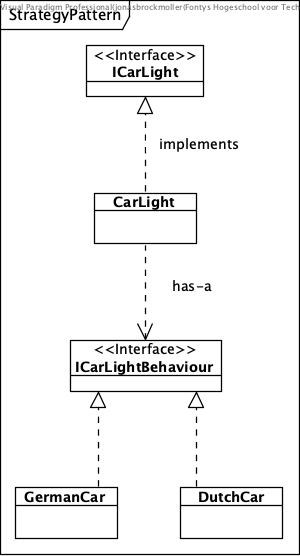
\includegraphics{pictures/StrategyPattern.png}
            \caption{Strategy pattern}
            \label{fig:strategyPattern}
        \end{minipage}%
        \hfill
        \begin{minipage}[b]{0.4\textwidth}
            \centering
            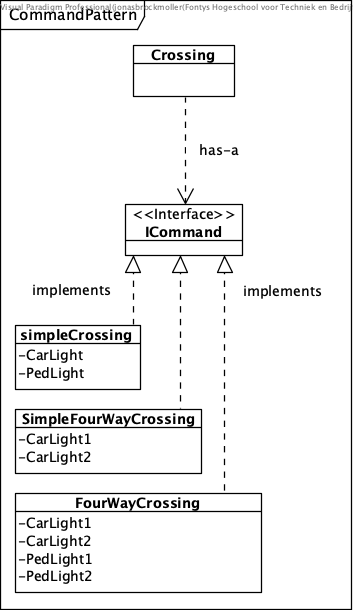
\includegraphics[scale=0.91]{pictures/CommandPattern.png}
            \caption{Command Pattern}
            \label{fig:commandPattern}
        \end{minipage}
    \end{figure}
    \begin{figure}[H]
        \centering
        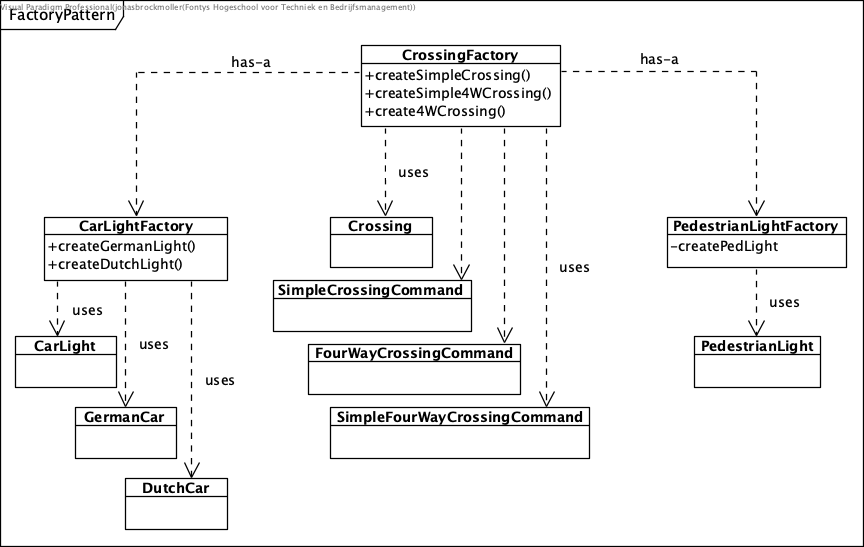
\includegraphics[scale=0.9]{pictures/FactoryPattern.png}
        \caption{Factory Pattern}
        \label{fig:factoryPattern}
    \end{figure}
    \begin{figure}[H]
        \centering
        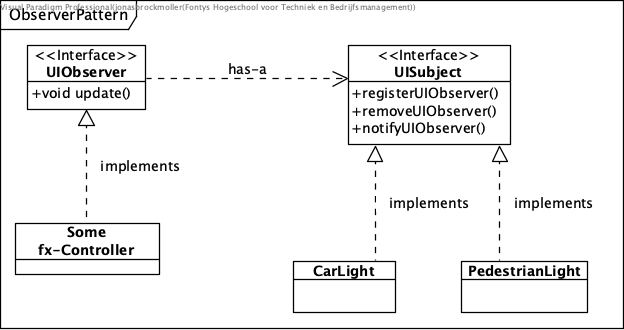
\includegraphics{pictures/ObserverPattern.png}
        \caption{Observer Pattern}
        \label{fig:observerPattern}
    \end{figure}
\end{document}
